% Created by tikzDevice version 0.12.6 on 2026-10-30 11:41:19
% !TEX encoding = UTF-8 Unicode
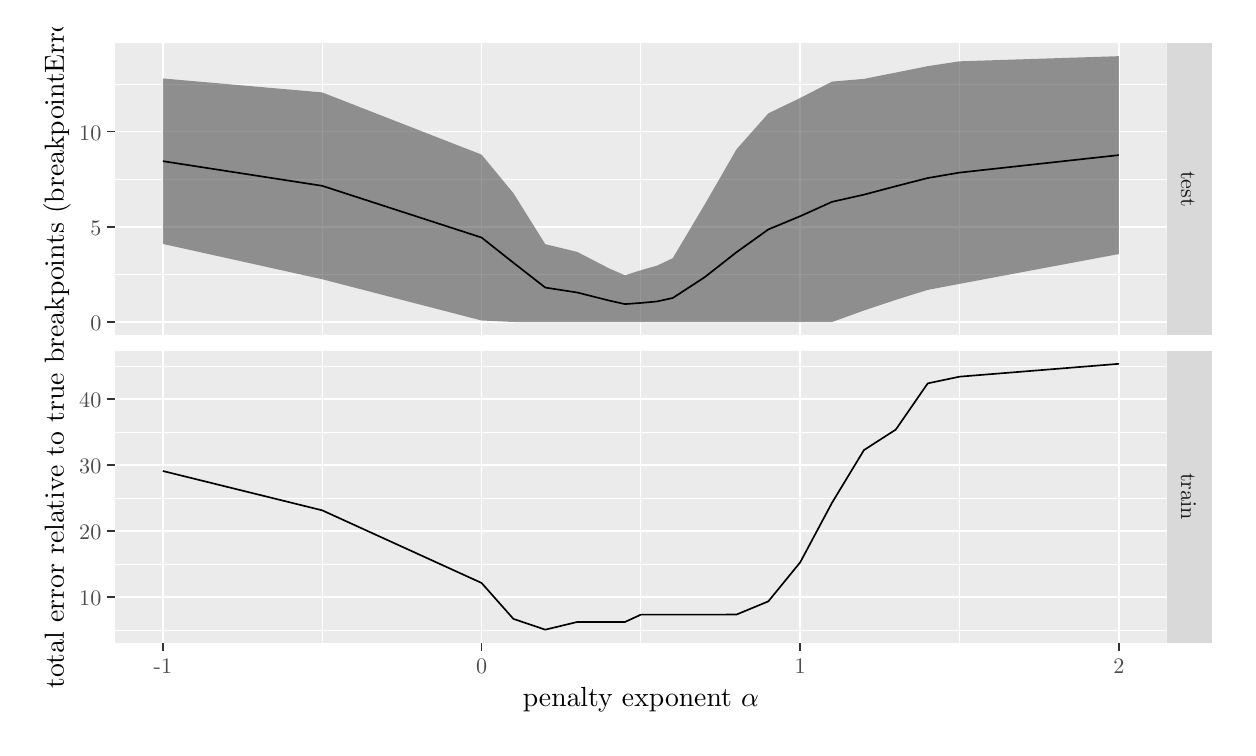
\begin{tikzpicture}[x=1pt,y=1pt]
\definecolor{fillColor}{RGB}{255,255,255}
\path[use as bounding box,fill=fillColor,fill opacity=0.00] (0,0) rectangle (433.62,252.94);
\begin{scope}
\path[clip] (  0.00,  0.00) rectangle (433.62,252.94);
\definecolor{drawColor}{RGB}{255,255,255}
\definecolor{fillColor}{RGB}{255,255,255}

\path[draw=drawColor,line width= 0.6pt,line join=round,line cap=round,fill=fillColor] (  0.00,  0.00) rectangle (433.62,252.94);
\end{scope}
\begin{scope}
\path[clip] ( 31.58,141.78) rectangle (411.58,247.45);
\definecolor{fillColor}{gray}{0.92}

\path[fill=fillColor] ( 31.58,141.78) rectangle (411.58,247.45);
\definecolor{drawColor}{RGB}{255,255,255}

\path[draw=drawColor,line width= 0.3pt,line join=round] ( 31.58,163.77) --
	(411.58,163.77);

\path[draw=drawColor,line width= 0.3pt,line join=round] ( 31.58,198.17) --
	(411.58,198.17);

\path[draw=drawColor,line width= 0.3pt,line join=round] ( 31.58,232.56) --
	(411.58,232.56);

\path[draw=drawColor,line width= 0.3pt,line join=round] (106.43,141.78) --
	(106.43,247.45);

\path[draw=drawColor,line width= 0.3pt,line join=round] (221.58,141.78) --
	(221.58,247.45);

\path[draw=drawColor,line width= 0.3pt,line join=round] (336.73,141.78) --
	(336.73,247.45);

\path[draw=drawColor,line width= 0.6pt,line join=round] ( 31.58,146.58) --
	(411.58,146.58);

\path[draw=drawColor,line width= 0.6pt,line join=round] ( 31.58,180.97) --
	(411.58,180.97);

\path[draw=drawColor,line width= 0.6pt,line join=round] ( 31.58,215.36) --
	(411.58,215.36);

\path[draw=drawColor,line width= 0.6pt,line join=round] ( 48.85,141.78) --
	( 48.85,247.45);

\path[draw=drawColor,line width= 0.6pt,line join=round] (164.01,141.78) --
	(164.01,247.45);

\path[draw=drawColor,line width= 0.6pt,line join=round] (279.16,141.78) --
	(279.16,247.45);

\path[draw=drawColor,line width= 0.6pt,line join=round] (394.31,141.78) --
	(394.31,247.45);
\definecolor{fillColor}{RGB}{51,51,51}

\path[fill=fillColor,fill opacity=0.50] ( 48.85,234.59) --
	(106.43,229.54) --
	(164.01,207.07) --
	(175.52,193.12) --
	(187.04,174.70) --
	(198.55,171.92) --
	(210.07,165.97) --
	(215.82,163.46) --
	(221.58,165.29) --
	(227.34,166.92) --
	(233.10,169.65) --
	(244.61,189.00) --
	(256.13,208.98) --
	(267.64,221.98) --
	(279.16,227.53) --
	(290.67,233.46) --
	(302.19,234.44) --
	(313.70,236.72) --
	(325.22,239.03) --
	(336.73,240.78) --
	(394.31,242.64) --
	(394.31,171.14) --
	(336.73,160.36) --
	(325.22,158.18) --
	(313.70,154.59) --
	(302.19,150.75) --
	(290.67,146.58) --
	(279.16,146.58) --
	(267.64,146.58) --
	(256.13,146.58) --
	(244.61,146.58) --
	(233.10,146.58) --
	(227.34,146.58) --
	(221.58,146.58) --
	(215.82,146.58) --
	(210.07,146.58) --
	(198.55,146.58) --
	(187.04,146.58) --
	(175.52,146.58) --
	(164.01,147.13) --
	(106.43,162.03) --
	( 48.85,174.80) --
	cycle;

\path[] ( 48.85,234.59) --
	(106.43,229.54) --
	(164.01,207.07) --
	(175.52,193.12) --
	(187.04,174.70) --
	(198.55,171.92) --
	(210.07,165.97) --
	(215.82,163.46) --
	(221.58,165.29) --
	(227.34,166.92) --
	(233.10,169.65) --
	(244.61,189.00) --
	(256.13,208.98) --
	(267.64,221.98) --
	(279.16,227.53) --
	(290.67,233.46) --
	(302.19,234.44) --
	(313.70,236.72) --
	(325.22,239.03) --
	(336.73,240.78) --
	(394.31,242.64);

\path[] (394.31,171.14) --
	(336.73,160.36) --
	(325.22,158.18) --
	(313.70,154.59) --
	(302.19,150.75) --
	(290.67,146.58) --
	(279.16,146.58) --
	(267.64,146.58) --
	(256.13,146.58) --
	(244.61,146.58) --
	(233.10,146.58) --
	(227.34,146.58) --
	(221.58,146.58) --
	(215.82,146.58) --
	(210.07,146.58) --
	(198.55,146.58) --
	(187.04,146.58) --
	(175.52,146.58) --
	(164.01,147.13) --
	(106.43,162.03) --
	( 48.85,174.80);
\definecolor{drawColor}{RGB}{0,0,0}

\path[draw=drawColor,line width= 0.6pt,line join=round] ( 48.85,204.70) --
	(106.43,195.79) --
	(164.01,177.10) --
	(175.52,167.99) --
	(187.04,159.02) --
	(198.55,157.25) --
	(210.07,154.34) --
	(215.82,153.05) --
	(221.58,153.47) --
	(227.34,154.00) --
	(233.10,155.26) --
	(244.61,162.75) --
	(256.13,171.80) --
	(267.64,180.03) --
	(279.16,184.82) --
	(290.67,190.01) --
	(302.19,192.60) --
	(313.70,195.65) --
	(325.22,198.60) --
	(336.73,200.57) --
	(394.31,206.89);
\end{scope}
\begin{scope}
\path[clip] ( 31.58, 30.61) rectangle (411.58,136.28);
\definecolor{fillColor}{gray}{0.92}

\path[fill=fillColor] ( 31.58, 30.61) rectangle (411.58,136.28);
\definecolor{drawColor}{RGB}{255,255,255}

\path[draw=drawColor,line width= 0.3pt,line join=round] ( 31.58, 35.29) --
	(411.58, 35.29);

\path[draw=drawColor,line width= 0.3pt,line join=round] ( 31.58, 59.14) --
	(411.58, 59.14);

\path[draw=drawColor,line width= 0.3pt,line join=round] ( 31.58, 83.00) --
	(411.58, 83.00);

\path[draw=drawColor,line width= 0.3pt,line join=round] ( 31.58,106.86) --
	(411.58,106.86);

\path[draw=drawColor,line width= 0.3pt,line join=round] ( 31.58,130.71) --
	(411.58,130.71);

\path[draw=drawColor,line width= 0.3pt,line join=round] (106.43, 30.61) --
	(106.43,136.28);

\path[draw=drawColor,line width= 0.3pt,line join=round] (221.58, 30.61) --
	(221.58,136.28);

\path[draw=drawColor,line width= 0.3pt,line join=round] (336.73, 30.61) --
	(336.73,136.28);

\path[draw=drawColor,line width= 0.6pt,line join=round] ( 31.58, 47.21) --
	(411.58, 47.21);

\path[draw=drawColor,line width= 0.6pt,line join=round] ( 31.58, 71.07) --
	(411.58, 71.07);

\path[draw=drawColor,line width= 0.6pt,line join=round] ( 31.58, 94.93) --
	(411.58, 94.93);

\path[draw=drawColor,line width= 0.6pt,line join=round] ( 31.58,118.78) --
	(411.58,118.78);

\path[draw=drawColor,line width= 0.6pt,line join=round] ( 48.85, 30.61) --
	( 48.85,136.28);

\path[draw=drawColor,line width= 0.6pt,line join=round] (164.01, 30.61) --
	(164.01,136.28);

\path[draw=drawColor,line width= 0.6pt,line join=round] (279.16, 30.61) --
	(279.16,136.28);

\path[draw=drawColor,line width= 0.6pt,line join=round] (394.31, 30.61) --
	(394.31,136.28);
\definecolor{drawColor}{RGB}{0,0,0}

\path[draw=drawColor,line width= 0.6pt,line join=round] ( 48.85, 92.74) --
	(106.43, 78.53) --
	(164.01, 52.29) --
	(175.52, 39.30) --
	(187.04, 35.41) --
	(198.55, 38.18) --
	(210.07, 38.18) --
	(215.82, 38.18) --
	(221.58, 40.84) --
	(227.34, 40.84) --
	(233.10, 40.84) --
	(244.61, 40.84) --
	(256.13, 40.87) --
	(267.64, 45.64) --
	(279.16, 59.76) --
	(290.67, 81.30) --
	(302.19,100.30) --
	(313.70,107.71) --
	(325.22,124.40) --
	(336.73,126.83) --
	(394.31,131.47);
\end{scope}
\begin{scope}
\path[clip] (411.58,141.78) rectangle (428.12,247.45);
\definecolor{fillColor}{gray}{0.85}

\path[fill=fillColor] (411.58,141.78) rectangle (428.12,247.45);
\definecolor{drawColor}{gray}{0.10}

\node[text=drawColor,rotate=-90.00,anchor=base,inner sep=0pt, outer sep=0pt, scale=  0.80] at (416.84,194.61) {test};
\end{scope}
\begin{scope}
\path[clip] (411.58, 30.61) rectangle (428.12,136.28);
\definecolor{fillColor}{gray}{0.85}

\path[fill=fillColor] (411.58, 30.61) rectangle (428.12,136.28);
\definecolor{drawColor}{gray}{0.10}

\node[text=drawColor,rotate=-90.00,anchor=base,inner sep=0pt, outer sep=0pt, scale=  0.80] at (416.84, 83.44) {train};
\end{scope}
\begin{scope}
\path[clip] (  0.00,  0.00) rectangle (433.62,252.94);
\definecolor{drawColor}{gray}{0.20}

\path[draw=drawColor,line width= 0.6pt,line join=round] ( 48.85, 27.86) --
	( 48.85, 30.61);

\path[draw=drawColor,line width= 0.6pt,line join=round] (164.01, 27.86) --
	(164.01, 30.61);

\path[draw=drawColor,line width= 0.6pt,line join=round] (279.16, 27.86) --
	(279.16, 30.61);

\path[draw=drawColor,line width= 0.6pt,line join=round] (394.31, 27.86) --
	(394.31, 30.61);
\end{scope}
\begin{scope}
\path[clip] (  0.00,  0.00) rectangle (433.62,252.94);
\definecolor{drawColor}{gray}{0.30}

\node[text=drawColor,anchor=base,inner sep=0pt, outer sep=0pt, scale=  0.80] at ( 48.85, 19.62) {-1};

\node[text=drawColor,anchor=base,inner sep=0pt, outer sep=0pt, scale=  0.80] at (164.01, 19.62) {0};

\node[text=drawColor,anchor=base,inner sep=0pt, outer sep=0pt, scale=  0.80] at (279.16, 19.62) {1};

\node[text=drawColor,anchor=base,inner sep=0pt, outer sep=0pt, scale=  0.80] at (394.31, 19.62) {2};
\end{scope}
\begin{scope}
\path[clip] (  0.00,  0.00) rectangle (433.62,252.94);
\definecolor{drawColor}{gray}{0.30}

\node[text=drawColor,anchor=base east,inner sep=0pt, outer sep=0pt, scale=  0.80] at ( 26.63,143.56) {0};

\node[text=drawColor,anchor=base east,inner sep=0pt, outer sep=0pt, scale=  0.80] at ( 26.63,177.95) {5};

\node[text=drawColor,anchor=base east,inner sep=0pt, outer sep=0pt, scale=  0.80] at ( 26.63,212.35) {10};
\end{scope}
\begin{scope}
\path[clip] (  0.00,  0.00) rectangle (433.62,252.94);
\definecolor{drawColor}{gray}{0.20}

\path[draw=drawColor,line width= 0.6pt,line join=round] ( 28.83,146.58) --
	( 31.58,146.58);

\path[draw=drawColor,line width= 0.6pt,line join=round] ( 28.83,180.97) --
	( 31.58,180.97);

\path[draw=drawColor,line width= 0.6pt,line join=round] ( 28.83,215.36) --
	( 31.58,215.36);
\end{scope}
\begin{scope}
\path[clip] (  0.00,  0.00) rectangle (433.62,252.94);
\definecolor{drawColor}{gray}{0.30}

\node[text=drawColor,anchor=base east,inner sep=0pt, outer sep=0pt, scale=  0.80] at ( 26.63, 44.20) {10};

\node[text=drawColor,anchor=base east,inner sep=0pt, outer sep=0pt, scale=  0.80] at ( 26.63, 68.05) {20};

\node[text=drawColor,anchor=base east,inner sep=0pt, outer sep=0pt, scale=  0.80] at ( 26.63, 91.91) {30};

\node[text=drawColor,anchor=base east,inner sep=0pt, outer sep=0pt, scale=  0.80] at ( 26.63,115.77) {40};
\end{scope}
\begin{scope}
\path[clip] (  0.00,  0.00) rectangle (433.62,252.94);
\definecolor{drawColor}{gray}{0.20}

\path[draw=drawColor,line width= 0.6pt,line join=round] ( 28.83, 47.21) --
	( 31.58, 47.21);

\path[draw=drawColor,line width= 0.6pt,line join=round] ( 28.83, 71.07) --
	( 31.58, 71.07);

\path[draw=drawColor,line width= 0.6pt,line join=round] ( 28.83, 94.93) --
	( 31.58, 94.93);

\path[draw=drawColor,line width= 0.6pt,line join=round] ( 28.83,118.78) --
	( 31.58,118.78);
\end{scope}
\begin{scope}
\path[clip] (  0.00,  0.00) rectangle (433.62,252.94);
\definecolor{drawColor}{RGB}{0,0,0}

\node[text=drawColor,anchor=base,inner sep=0pt, outer sep=0pt, scale=  1.00] at (221.58,  7.63) {penalty exponent $\alpha$};
\end{scope}
\begin{scope}
\path[clip] (  0.00,  0.00) rectangle (433.62,252.94);
\definecolor{drawColor}{RGB}{0,0,0}

\node[text=drawColor,rotate= 90.00,anchor=base,inner sep=0pt, outer sep=0pt, scale=  1.00] at ( 13.04,139.03) {total error relative to true breakpoints (breakpointError)};
\end{scope}
\end{tikzpicture}
